% \newpage
%
\subsection{Инвентаризация материалов}
%\label{bp:MatOutput}

 Инвентаризация материалов проводится один раз в год. Ежегодно выпускается приказ о проведении инвентаризации.
% (рис. \ref{pic:Инвентаризация приказ}).
Согласно приказу создаются комиссии. В 1С: УПП оформляются документы:''Инвентаризационная ведомость'', ''Сличительная ведомость'' (рис. \ref{pic:Слич ведомость}). По результатам проведения инвентаризации в 1С: УПП оформляются документы по списанию и поступлению ТМЦ.  





% \begin{figure}
% \begin{center}
%  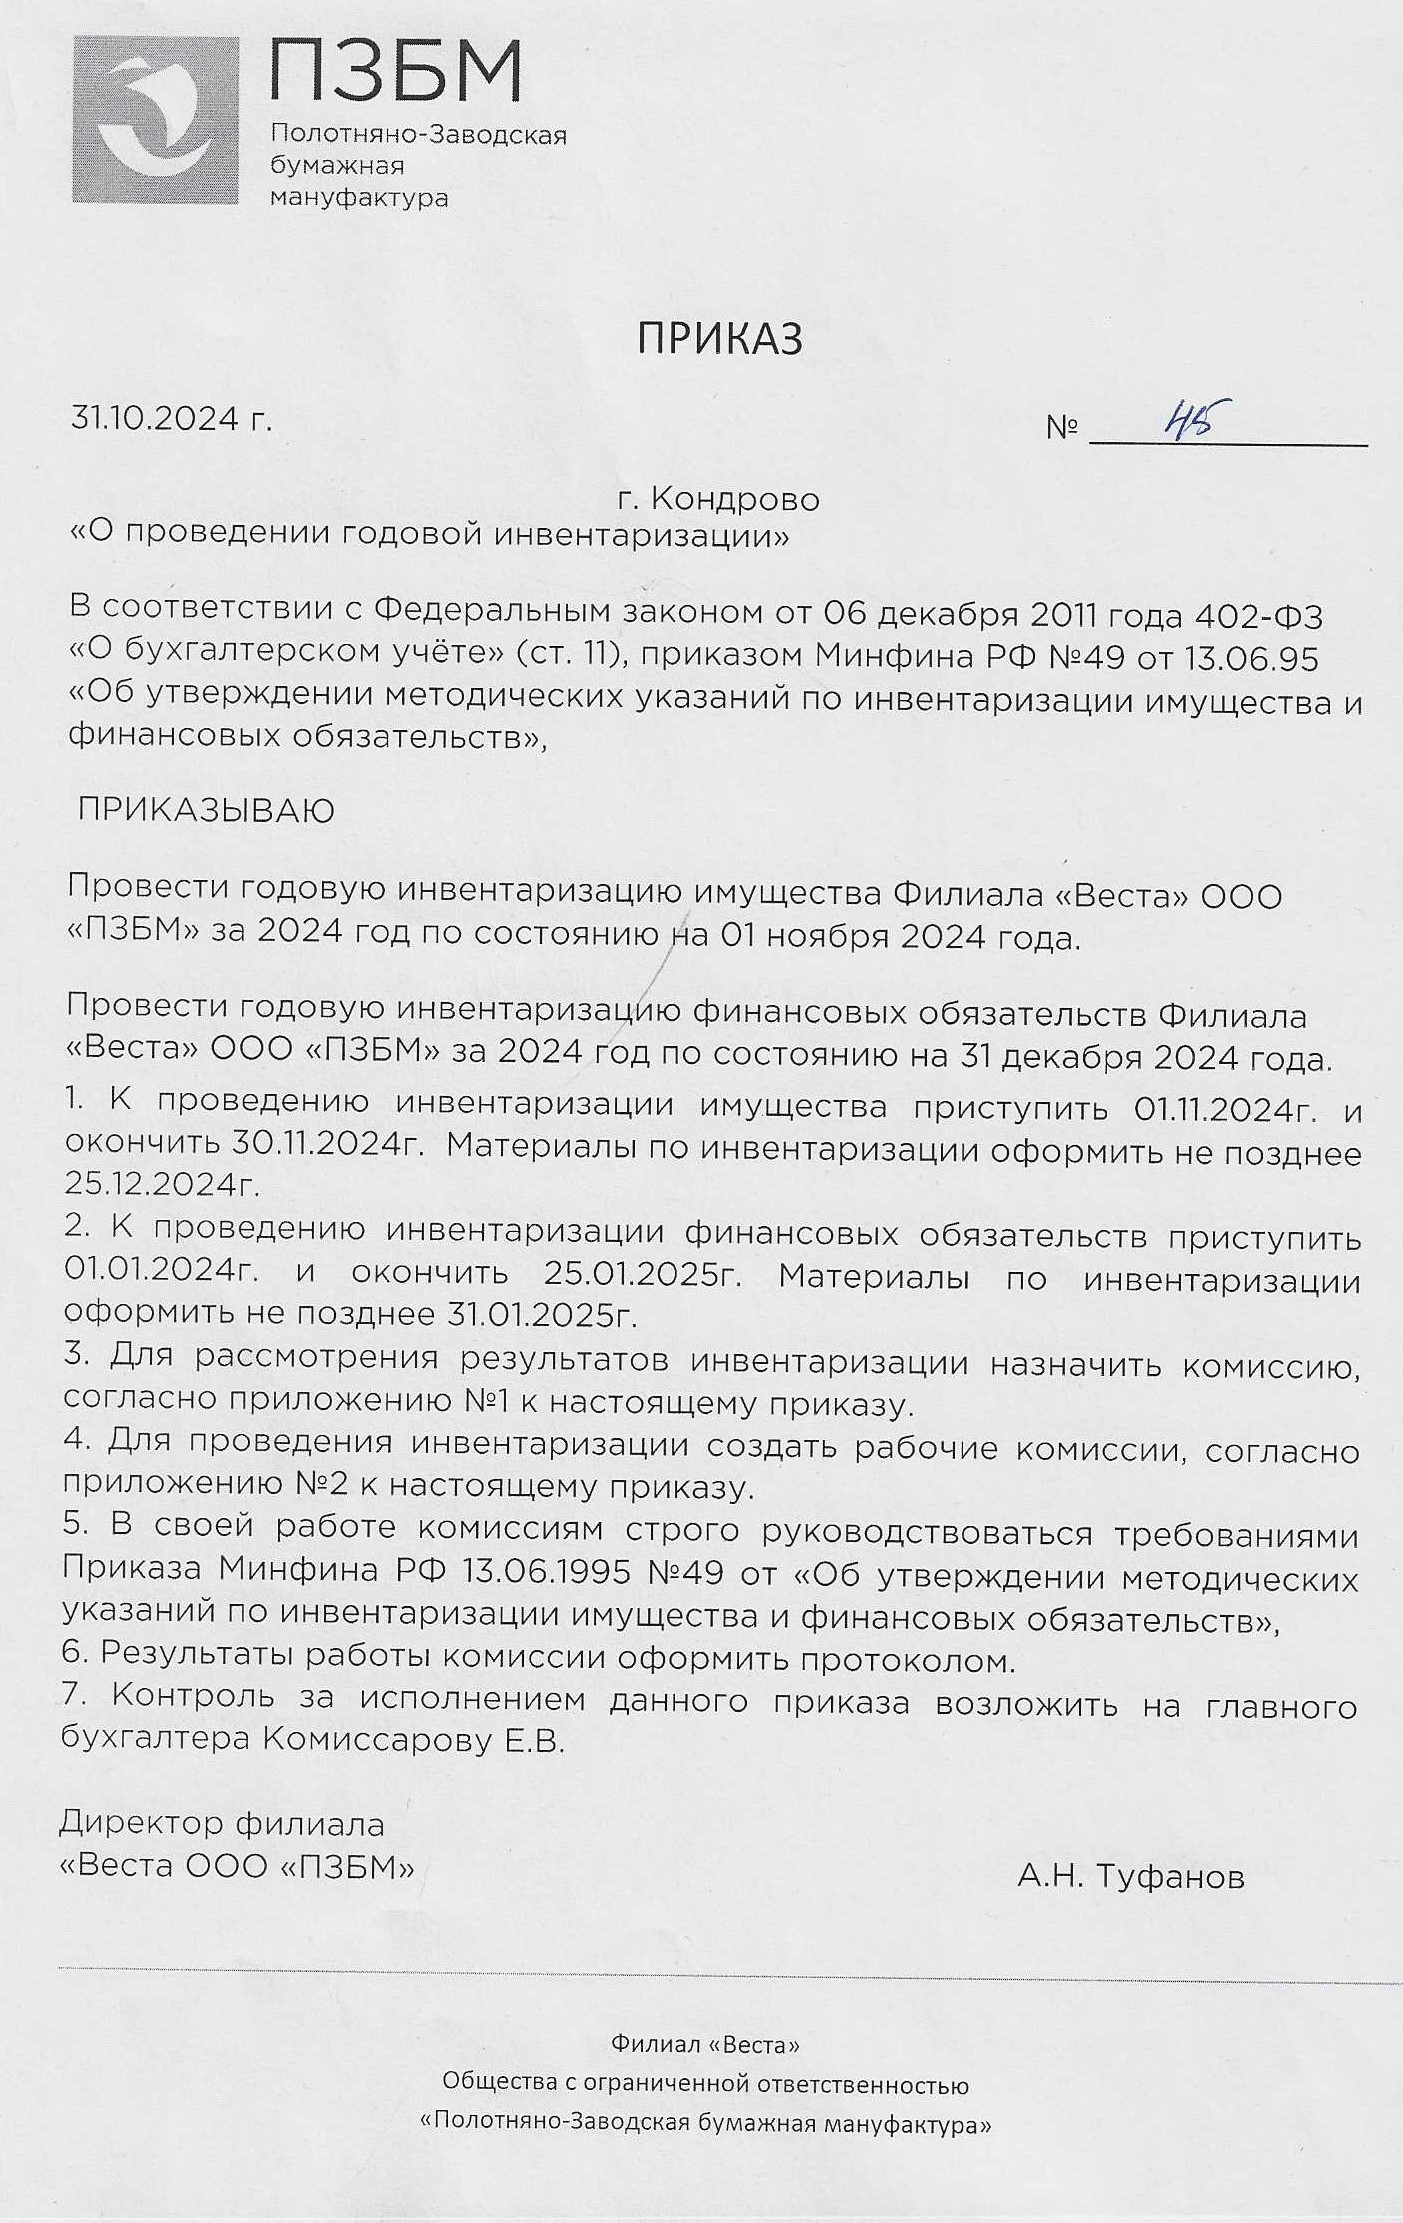
\includegraphics[height=0.9\textheight, keepaspectratio]{Pics/Инвентаризация приказ.jpg}
% \end{center}
%  \caption{Приказ о проведении инвентаризации}
%  \label{pic:Инвентаризация приказ}
% \end{figure}

\begin{figure}
\begin{center}
 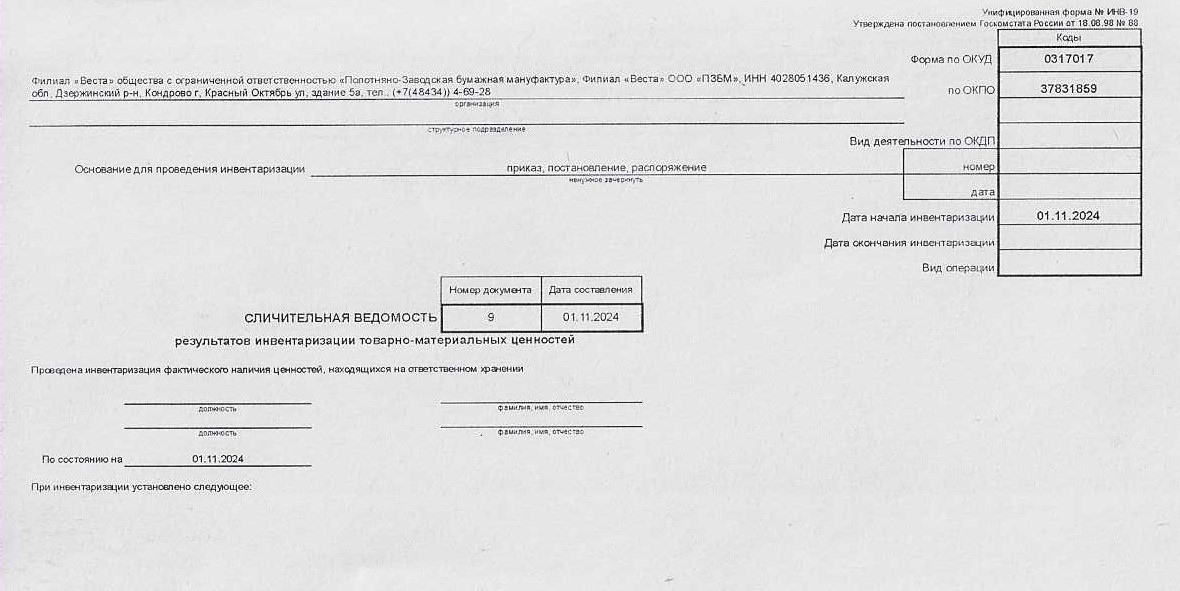
\includegraphics[height=0.33\textheight, keepaspectratio]{Pics/Слич ведомость.jpg}
\end{center}
 \caption{Сличительная ведомость}
 \label{pic:Слич ведомость}
\end{figure}
%Инвентаризация по готовой продукции проводится каждый месяц на основании данных учета в системе СБИС.

 \clearpage
\ifx \notincludehead\undefined
\normalsize
\end{document}
\fi